\newpage
安排
\begin{enumerate}
    \item 深度学习基础
    \item 神经网络基础类型
    \item 计算机视觉与自然语言处理
    \item 基于深度学习三维点云理解
    \item 基于深度学习的蛋白质识别
    \item 生成模型(一)
    \item 生成模型(二)
    \item 具身(embodied)人工智能简介
\end{enumerate}

大作业ppt要求:
\begin{enumerate}\small
    \item 	任务与数据集介绍(10分); 任务难易程度(5分), 鼓励尝试具有挑战的前沿课题; 
    \item 输入, 神经网络结构, 输出, 损失函数, 训练过程介绍(30分); 
    \item 代码实现(30分) (完整的代码以及详细的ReadMe文件, 确保代码能够顺利跑通); 
    \item 成果, 性能展示(性能高低不计入评分标准)(20分); 
    \item 结果可视化, 新问题发现, 已有问题解决, 方法创新以及任何其他亮点(5分).     
\end{enumerate}

大作业代码要求:
\begin{enumerate}
    \item dataset 数据集 自己写
    \item models 网络结构 自己写
    \item modules 可以调其他的包, 比如说 \href{https://github.com/hehefan/P4Transformer/tree/main/modules-pytorch-1.4.0}{P4Transformer} (点云处理)
    \item train.py 就 train
    \item utils.py 一些操作, 不属于上列的都塞到这里
\end{enumerate}

\section{深度学习基础}

\subsection{发展历程}
基于规则或基于学习 

AlexNet(2012)

\subsection{神经网络基础知识}
人工神经网络+训练学习策略

统计机器学习: 找规律, 有 pattern (拟合极小规模数据去验证网络的合理性)
\begin{align*}
    \hat{y}\ \ y=f(x;\theta)
\end{align*}

\subsubsection{网络类型}
$f(\cdot; \theta)$:
\begin{enumerate}
    \item 多层感知机 (MLP): $>3$层, 单层就叫fc即可
    \item 卷积神经网络 (CNN): 局部特征带有噪声
    \item 循环神经网络 (RNN): 越后期的输入影响越大
    \item Transformer: 自注意力 
    \begin{figure}[!htb]
        \centering
        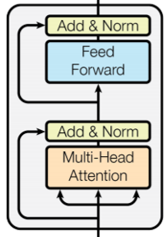
\includegraphics[width=0.14\textwidth]{pic/DL1/Transformer.png}
        \caption{Transformer}
    \end{figure}
    
    \item 图网路 (GNN): 顶点与边都是特征
\end{enumerate}

deep neural network (parameterized function): operation $\rightarrow$ architecture

\subsubsection{数据}
$x$:
\begin{enumerate}
    \item 一维: 声音, 文本
    \item 二维: 图像
    \item 三维: 点云, 结构
\end{enumerate}

\subsubsection{任务}
$y$:
\begin{enumerate}
    \item 分类
    \item 语义分割
    \item 目标检测
    \item 生成
\end{enumerate}

\subsubsection{训练}
$\hat{y}$, e.g.
\begin{enumerate}
    \item 监督学习: 数据有标签
    \item 无监督学习: 数据无标签, 要模型寻找数据内在联系
    \item 半监督学习: 部分数据有标签
    \item 弱监督学习: 数据有标签, 但有一定噪声
    \item 强化学习: 在线规划, 探索(在未知之中)与遵从(现有知识)寻找平衡, 有不可导的梯度时可以以此传递
\end{enumerate}



\subsection{基础学习算法介绍}
\subsubsection{数据}
\paragraph{图像}
规则有序, 位置离散的二维网格
\begin{align*}
    H\times W\times C \rightarrow 1\times 1\times C'
\end{align*}
$C' \gg C$

\paragraph{文本}
规则有序, 位置离散的列表
\begin{align*}
    v^T W \rightarrow S
\end{align*}
词典$v\in \mathbb{R}^{5\times 1}$, $W\in \mathbb{R}^{5\times 128}$, $S \in \mathbb{R}^{5\times 128}$

\paragraph{点云 (point cloud or point set)}
不规则无序的三维点集合 $P \in \mathbb{R}^{N\times 3}$, 点位置连续但点不连续

\paragraph{点云视频}
点集合列表, 三维点 (不规则, 无序, 位置连续)+一维时间 (规则有序, 位置离散)

\paragraph{蛋白质结构} 
点列表, 三维结构 (不规则, 无序, 位置连续)+一维结构 (规则有序, 位置离散)
\begin{enumerate}
    \item 一级
    \item 二级
    \item 三级
    \item 四级
\end{enumerate}

\subsection{大作业背景介绍}

Transformer 找相关区域, 然后对其进行编码找特征. 使用自注意力追踪. 

三维动作点云需要时空解耦


